    \documentclass[
        fleqn,
        usenatbib,
        % referee,
    ]{mnras}
    \usepackage{
        amsmath,
        amssymb,
        newtxtext,
        newtxmath,
        ae, aecompl,
        graphicx,
        booktabs,
        xcolor,
    }

    \newcommand*{\scinot}[2]{#1\times10^{#2}}
    \newcommand*{\rd}[2]{\frac{\mathrm{d}#1}{\mathrm{d}#2}}
    \newcommand*{\rtd}[2]{\frac{\mathrm{d}^2#1}{\mathrm{d}#2^2}}
    \newcommand*{\pd}[2]{\frac{\partial#1}{\partial#2}}
    \newcommand*{\ptd}[2]{\frac{\partial^2#1}{\partial#2^2}}
    % inline
    \newcommand*{\mdil}[2]{\mathrm{D}#1/\mathrm{D}#2}
    \newcommand*{\pdil}[2]{\partial#1/\partial#2}
    \newcommand*{\rdil}[2]{\mathrm{d}#1/\mathrm{d}#2}
    \newcommand*{\at}[1]{\left.#1\right|}
    \newcommand*{\abs}[1]{\left|#1\right|}
    \newcommand*{\ev}[1]{\left\langle#1\right\rangle}
    \newcommand*{\p}[1]{\left(#1\right)}
    \newcommand*{\s}[1]{\left[#1\right]}
    \newcommand*{\z}[1]{\left\{#1\right\}}
    \newcommand*{\bm}[1]{\mathbf{#1}}
    \newcommand*{\uv}[1]{\hat{\mathbf{#1}}}
    \newcommand*{\md}[0]{\mathrm{d}}
    \DeclareMathOperator*{\med}{med}
    \DeclareMathOperator*{\erf}{erf}

\title[Weak Tides and Cassini States]{Dynamics of Colombo's Top: Tidal
Dissipation and Resonance Capture}
\author[Y. Su and D. Lai.]{
Yubo Su,$^1$\thanks{E-mail: yubosu@astro.cornell.edu},
Dong Lai$^{1,2}$
\\
$^1$ Cornell Center for Astrophysics and Planetary Science, Department of
Astronomy, Cornell University, Ithaca, NY 14853, USA\\
$^2$ Tsung-Dao Lee Institute \& School of Physics and Astronomy, Shanghai Jiao
Tong University, 200240 Shanghai, China
}

\date{Accepted XXX\@. Received YYY\@; in original form ZZZ}

\pubyear{2021}

\begin{document}\label{firstpage}
\pagerange{\pageref{firstpage}--\pageref{lastpage}}
\maketitle

\begin{abstract}
    Abstract here
\end{abstract}

\begin{keywords}
planet-star interactions
\end{keywords}

\section{Introduction}\label{s:intro}

\begin{itemize}
    \item Studying planetary obliquities (define) is important. Cassini States
        are key. More introduction.

    \item Resonance capture via separatrix crossing was first considered by
        \citep{henrard1982} for non-dissipative perturbations
        \citep[e.g.][]{su2020}. However, tidal friction is dissipative, so this
        formalism does not apply. We generalize this calculation and show that
        it reproduces results.
\end{itemize}

In Section XXX\dots

\section{Spin Evolution Equations and Cassini States: Review}\label{s:theory}

In this section, we first briefly lay out the spin dynamics of the planet,
introducing the Cassini State spin-orbit resonance \citep[for more details,
see][]{su2020}. We then introduce the weak friction theory of equilibrium tides
used in this work \citep{lai2012}. While many different tidal effects may
dominate in different planetary systems, our qualitative conclusions do not
depend on the specific form of the tidal dissipation, so we use the classic weak
friction theory for simplicity.

\subsection{Spin Dynamics in the Absence of Tides}\label{ss:theory_spin}

\subsubsection{Equations of Motion}

We consider a star of mass $M_\star$ hosting an inner oblate planet of mass $m$
and radius $R$ on a circular orbit with semi-major axis $a$ and an outer
perturber of mass $m_{\rm p}$ on a circular orbit with semi-major axis $a_{\rm
p}$. We assume that the two orbits are mildly misaligned with mutual inclination
$I$. Denote $\bm{S}$ the spin angular momentum and $\bm{L}$ the orbital angular
momentum of the planet, and $\bm{L}_{\rm p}$ the angular momentum of the
perturber. The corresponding unit vectors are $\uv{s} \equiv \bm{S} / S$,
$\uv{l} \equiv \bm{L} / L$, and $\uv{l}_{\rm p} \equiv \bm{L}_{\rm p} / L_{\rm
p}$. The spin axis $\uv{s}$ of the planet tends to precess around its orbital
(angular momentum) axis $\uv{l}$, driven by the gravitational torque from the
host star acting on the planet's rotational bulge. On the other hand, $\uv{l}$
and the disk axis $\uv{l}_{\rm p}$ precess around each other due to
gravitational interactions. We assume $S \ll L \ll L_{\rm p}$, so $\uv{l}_{\rm
p}$ and $\uv{l}$ are nearly constant. The equations of motion for $\uv{s}$ and
$\uv{l}$ in this limit are \citep{anderson2018teeter, su2020}
\begin{align}
    \rd{\uv{s}}{t}
        &= \omega_{\rm sl}\p{\uv{s} \cdot \uv{l}}\p{\uv{s} \times \uv{l}}
        \equiv \alpha\p{\uv{s} \cdot \uv{l}}\p{\uv{s} \times
        \uv{l}},\label{eq:dsdt1}\\
    \rd{\uv{l}}{t} &= \omega_{\rm lp}\p{\uv{l} \cdot \uv{l}_{\rm p}}\p{\uv{l}
        \times \uv{l}_{\rm p}} \equiv -g\p{\uv{l} \times \uv{l}_{\rm p}},
        \label{eq:dldt1}
\end{align}
where
\begin{align}
    \omega_{\rm sl} &\equiv \frac{3GJ_2 mR^2 M_\star}{2a^3 I\Omega_{\rm s}}
        = \frac{3k_q}{2k}\frac{M_\star}{m}\p{\frac{R}{a}}^3 \Omega_{\rm s},
            \label{eq:wsl}\\
    \omega_{\rm lp} &= \frac{3m_p}{4M_\star}\p{\frac{a}{a_{\rm p}}}^3
        n.\label{eq:wlp}
\end{align}
In Eq.~\eqref{eq:wsl}, $\Omega_{\rm s}$ is the spin frequency of the inner
planet, $I = k mR^2$ (with $k$ a constant) is its moment of inertia and $J_2 =
k_{\rm q}\Omega_{\rm s}^2 (R^3/Gm)$ (with $k_{q}$ a constant) is its rotation-induced
(dimensionless) quadrupole moment [for a body with uniform density, $k=0.4,
k_{\rm q}=0.5$; for rocky planets, $k\simeq 0.2$ and $k_{\rm q}\simeq 0.17$
\citep[e.g.][]{lainey2016quantification} \textcolor{red}{? not sure}]. In other
studies, $3k_{\rm q} / 2 k$ is often notated as $k_2 / 2C$
\citep[e.g.][]{millholland_disk}. In Eq.~\eqref{eq:wlp}, $n \equiv
\sqrt{GM_\star/a^3}$ is the inner planet's orbital mean motion,  and we have
assumed $a_{\rm p}\gg a$ and included only the leading-order (quadrupole)
interaction between the inner planet and perturber. Following standard notation,
we define $\alpha = \omega_{\rm sl}$ and $g \equiv -\omega_{\rm 1p} \cos I$
\citep[e.g.][]{colombo1966}.

As in \citet{su2020}, we combine Eqs.~(\ref{eq:dsdt1}--\ref{eq:dldt1}) into a
single equation by transforming into a frame rotating about $\uv{l}_{\rm p}$
with frequency $g$. In this frame, $\uv{l}_{\rm p}$ and $\uv{l}$ are both fixed,
and $\uv{s}$ evolves as:
\begin{equation}
    \p{\rd{\uv{s}}{t}}_{\rm rot}
        = \alpha\p{\uv{s} \cdot \uv{l}}\p{\uv{s} \times \uv{l}}
            + g\p{\uv{s} \times \uv{l}_{\rm p}}. \label{eq:dsdt_rot}
\end{equation}
In this reference frame, we choose the coordinate system such that $\uv{z} =
\uv{l}$ and $\uv{l}_{\rm p}$ lies in the $\uv{x}$-$\uv{z}$ plane. We describe
$\uv{s}$ in spherical coordinates using the polar angle $\theta$, the planet's
obliquity, and $\phi$, the precessional phase of $\uv{s}$ about $\uv{l}$.

The equilibria of Eq.~\eqref{eq:dsdt_rot} are referred to as \emph{Cassini
States} \citep[CSs;][]{colombo1966, peale1969}. We follow the notation of
\citet{su2020}, where the parameter
\begin{equation}
    \eta \equiv -\frac{g}{\alpha},\label{eq:def_eta}
\end{equation}
is used. For a given value of $\eta$, there can be either two or four CSs, all
of which require $\uv{s}$ lie in the plane of $\uv{l}$ and $\uv{l}_{\rm p}$.
Following the standard convention and nomenclature, CSs 1, 3, and 4 have $\phi =
0$ and $\theta < 0$, while CS2 has $\phi = \pi$ and $\theta > 0$.
Figure~\ref{fig:cs_locs} shows the CS obliquities as a function of $\eta$, each
of which satisfies
\begin{equation}
    \sin \theta \cos \theta - \eta \sin\p{\theta - I} = 0.\label{eq:cs_zero}
\end{equation}
Note that there are four CSs when $\eta < \eta_{\rm c}$ and only two when $\eta
> \eta_{\rm c}$, where
\begin{equation}
    \eta_{\rm c} \equiv \p{\sin^{2/3}\!I + \cos^{2/3}\!I}^{-3/2}.\label{eq:def_etac}
\end{equation}
\begin{figure}
    \centering
    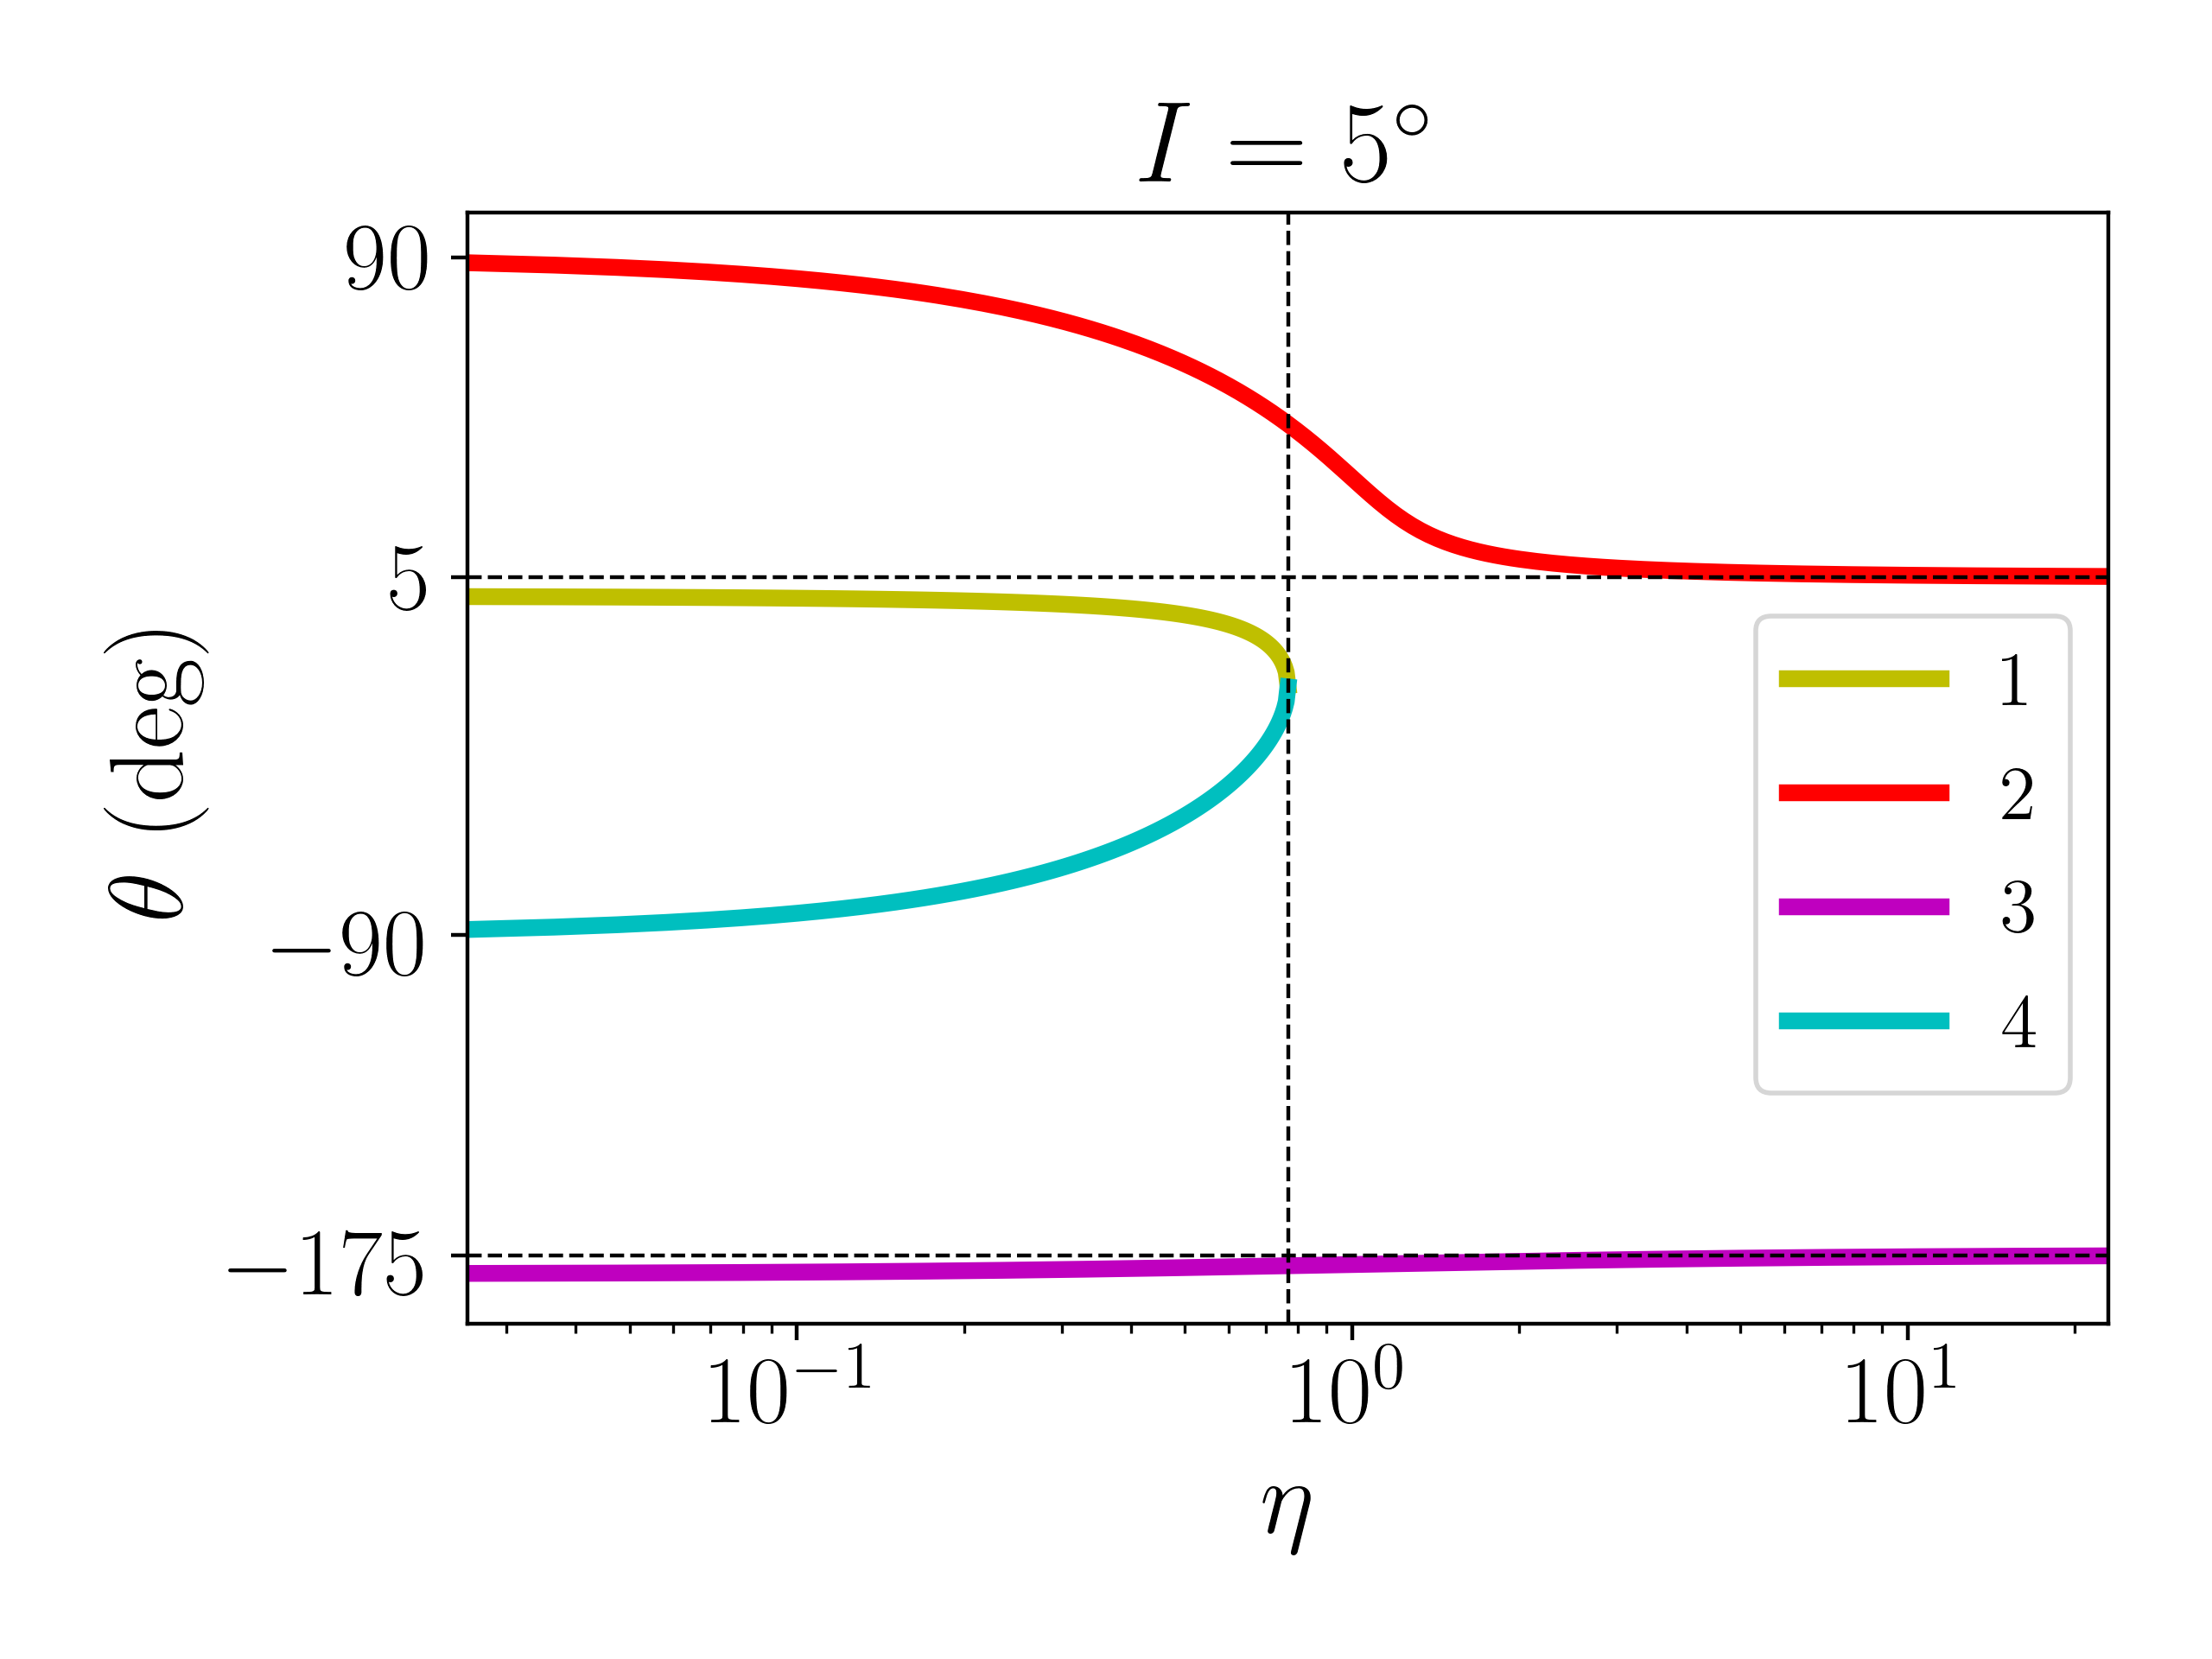
\includegraphics[width=\columnwidth]{../initial/99_misc/2_cs_locs.png}
    \caption{Cassini State obliquities $\theta$ as a function of $\eta \equiv
    -g/\alpha$ (Eq.~\ref{eq:def_eta}) for $I = 5^\circ$. The vertical dashed
    line denotes $\eta_{\rm c}$, where the number of Cassini States changes from
    four to just two (Eq.~\ref{eq:def_etac}). The horizontal dashed line gives
    $\theta = I$, the asymptotic value of Cassini State 2's obliquity when $\eta
    \to \infty$.}\label{fig:cs_locs}
\end{figure}

The Hamiltonian corresponding to Eq.~\eqref{eq:dsdt_rot} is
\begin{align}
    H &= -\frac{\alpha}{2}\p{\uv{s} \cdot \uv{l}}^2
            - g\p{\uv{s} \cdot \uv{l}_{\rm d}}\nonumber\\
        &= -\frac{\alpha}{2} \cos^2\theta
            - g\p{\cos\theta \cos I - \sin I \sin\theta \cos \phi}.\label{eq:H}
\end{align}
Here, $\cos \theta$ and $\phi$ form a canonically conjugate pair of variables.
Figure~\ref{fig:1contours} shows the level curves of this Hamiltonian for $I =
20^\circ$, for which $\eta_{\rm c} \approx 0.77$ (Eq.~\ref{eq:def_etac}). When $\eta
< \eta_{\rm c}$, CS4 exists and is a saddle point. The two trajectories
originating and ending at CS4 are the only two infinite-period orbits in the
phase space. Together, these two critical trajectories are referred to as the
\emph{separatrix} and divide phase space into three zones. Trajectories in zone
II librate about CS2 while those in zones I and III circulate. On the other
hand, when $\eta > \eta_{\rm c}$, all trajectories circulate. When the
separatrix exists, we divide it into two curves: $\mathcal{C}_+$, the boundary
between zones I and II, and $\mathcal{C}_-$, the boundary between zones II and
III\@.
\begin{figure}
    \centering
    \includegraphics[width=\columnwidth]{../initial/0_eta/1contours.png}
    \caption{Level curves of the Cassini State Hamiltonian (Eq.~\ref{eq:H}) for
    $I = 5^\circ$, for which $\eta_{\rm c} \approx 0.77$ (Eq.~\ref{eq:def_etac}).
    For $\eta < \eta_{\rm c}$, there are four Cassini States (labeled), while
    for $\eta > \eta_{\rm c}$ there are only two. In the former case, the
    existence of a \emph{separatrix} (solid black lines) separates phase space
    into three numbered zones (I/II/III, labeled). Finally, we denote the upper
    and lower legs of the separatrix by $\mathcal{C}_{\pm}$ respectively, as
    shown in the upper two panels.}\label{fig:1contours}
\end{figure}

\section{Spin Evolution with Alignment Torque}\label{s:toy_model}

In this section, we consider a simplified model of equilibrium tides that
isolates the important new phenomenon presented in this paper. We assume that
the spin magnitude of the planet is constant, so $\alpha$ and $g$ are both
fixed, while the spin orientation $\uv{s}$ experiences an alignment torque
towards $\uv{l}$ on the alignment timescale $t_{\rm s}$:
\begin{equation}
    \p{\rd{\uv{s}}{t}}_{\rm tide}
        = \frac{1}{t_{\rm s}} \uv{s} \times \p{\uv{l} \times \uv{s}}.
        \label{eq:dsdt_tide_toy}
\end{equation}
The full equations of motion for $\uv{s}$ in the coordinates $\theta$ and $\phi$
can be written:
\begin{align}
    \rd{\theta}{t} &= -g\sin I \sin \phi - \frac{1}{t_{\rm s}} \sin \theta,
        \label{eq:dqdt_toy}\\
    \rd{\phi}{t} &= -\alpha \cos\theta
        - g\p{\cos I + \sin I \cot \theta \cos \phi}.\label{eq:dfdt_toy}
\end{align}

\subsection{Shifted Cassini States and Linear Stability
Analysis}\label{ss:tidal_equils}

If the alignment torque is weak ($\abs{gt_{\rm s}} \gg 1$), then the fixed points of
Eqs.~(\ref{eq:dqdt_toy}--\ref{eq:dfdt_toy}) are just slightly shifted CSs. This
shift can be calculated cleanly to leading order: all of the CS obliquities
$\theta_{\rm cs}$ are unchanged while the azimuthal angle $\phi_{\rm cs}$ for
each CS now satisfies
\begin{equation}
    \sin \phi_{\rm cs} = \frac{\sin\theta_{\rm cs}}{\sin I \abs{g}t_{\rm s}}.
        \label{eq:mcs_shift}
\end{equation}
We can see that if $t_{\rm s} > t_{\rm s, c}$, where
\begin{align}
    t_{\rm s, c} &= \frac{1}{\abs{g}\sin I},
\end{align}
then Eq.~\eqref{eq:mcs_shift} will always have solutions for $\phi_{\rm cs}$,
and the alignment torque never changes the number of fixed points of the system.
If $t_{\rm s}$ is decreased below $t_{\rm s, c}$, CS2 and CS4 cease to be
fixed points if $\eta \ll 1$ \citep[as first noted in][]{fabrycky_otides}, as
$\theta_{\rm cs} \approx 90^\circ$ for these (see Fig.~\ref{fig:cs_locs}), while
the other CSs have small $\sin \theta_{\rm cs}$ and are only slightly perturbed.
Figure~\ref{fig:mcs} shows the obliquity and azimuthal angles for each of the
CSs in the $\eta \ll 1$ case, where it can be seen that CS2 and CS4 collide and
annihilate.. For the remainder of this section, we will consider the case where
$t_{\rm s} \gg t_{\rm s, c}$ and the CSs only differ slightly from their
unperturbed locations.
\begin{figure}
    \centering
    \includegraphics[width=\columnwidth]{../initial/99_misc/0_stab.png}
    \caption{Modified CSs for $I = 5^\circ$ and $\eta = 0.2$, and the CS1 and
    CS3 obliquities have been offset (labeled in legend) to improve clarity of
    the plot.}\label{fig:mcs}
\end{figure}

We next seek to characterize the stability of small perturbations about each of
the CSs in the presence of the weak tidal alignment torque. We can linearize
Eqs.~(\ref{eq:dqdt_toy}--\ref{eq:dfdt_toy}) about a shifted CS, yelding
\begin{align}
    \rd{}{t}\begin{bmatrix}
        \theta\\ \phi
    \end{bmatrix} &= \begin{bmatrix}
        -\frac{\cos \theta}{t_{\rm s}} &
        -g\sin I \cos \phi \\
        \alpha \sin \theta + g\frac{\sin I \cos \phi}{\sin^2\theta} &
        0
    \end{bmatrix}_{\rm cs}\begin{bmatrix}
        \Delta \theta \\ \Delta \phi
    \end{bmatrix},\label{eq:dsdt_hessian}
\end{align}
where the cs subscript indicates evaluating at a CS, $\Delta \theta = \theta -
\theta_{\rm cs}$, and $\Delta \phi = \phi - \phi_{\rm cs}$. The eigenvalues
$\lambda$ of Eq.~\eqref{eq:dsdt_hessian} satisfy the equation
\begin{align}
    0 &= \p{\lambda + \frac{\cos \theta_{\rm cs}}{t_{\rm s}}}\lambda - \lambda_0^2,\\
    \lambda_0^2 &\equiv \p{\alpha
        \sin \theta_{\rm cs} + g\sin I \csc^2\theta_{\rm cs}\cos \phi_{\rm cs}}
            \p{- g \sin I \cos \phi_{\rm cs}},\label{eq:def_l0_sq}\\
    \lambda &\approx -\frac{\cos \theta_{\rm cs}}{t_{\rm s}} \pm \sqrt{\lambda_0^2}.
        \label{eq:lambda_approx}
\end{align}
The stability depends only on the real part of $\lambda$ in
Eq.~\eqref{eq:lambda_approx}. $\lambda_0^2$ is a generalization of Eq.~(A4)
in, \citet{su2020} and generally has the same behavior: it is negative for CSs
1--3 and positive for CS4, as shown in Fig.~\ref{fig:lambda_full}. Thus, CS4 is
always unstable, as there will always be at least one positive solution for
$\lambda$, and the stability of CSs 1--3 are solely determined by the sign of
$\cos \theta_{\rm cs}$. From Figs.~\ref{fig:cs_locs}, we thus see that CSs 1 and
2 are stable while CS3 is unstable under the alignment torque. These
calculations justify results long used in CS literature
\citep[e.g.][]{ward1975tidal}.
\begin{figure}
    \centering
    \includegraphics[width=\columnwidth]{../initial/99_misc/2_lambdas_full.png}
    \caption{$\lambda_0^2$ (Eq.~\ref{eq:def_l0_sq}) as a function of $\eta
    \equiv \abs{g} / \alpha$ for the four CSs. The solid lines give
    $\lambda_0^2$ for the unperturbed $\phi_{\rm cs}$, and the dashed lines give
    the values for $\phi_{\rm cs}$ shifted by $60^\circ$ ($\phi_{\rm cs} =
    120^\circ$ for CS2 and $\phi_{\rm cs} = 60^\circ$ for CSs 1, 3, and 4).
    }\label{fig:lambda_full}
\end{figure}

\subsection{Spin Obliquity Evolution Driven by Alignment
Torque}\label{ss:toy_outcomes}

With the above results, we are equipped to ask questions about the dynamics of
Eqs.~(\ref{eq:dqdt_toy}--\ref{eq:dfdt_toy}): what is the long term behavior for
a general initial $\uv{s}$? If $\eta > \eta_{\rm c}$, then the only possible
final spin state is CS2, and all initial conditions will evolve asympotically
towards it. As such, we consider only $\eta < \eta_{\rm c}$, where an initial
condition can asymptotically evolve towards either CS1 or CS2. In
Fig.~\ref{fig:toy_phop}, we show which CS an initial $\theta_0$ and $\phi_0$
evolves into, where we have taken $\abs{g}t_{\rm s} = 10^{-3}$, $\eta = 0.2$,
and $I = 20^\circ$. It is clear that initial $\uv{s}$ in zone I (following the
naming in Fig.~\ref{fig:1contours}) evolve into CS1, those in zone II evolve
into CS2, while those in zone III have a probabilistic outcome. We aim to
understand each of these in turn:
\begin{figure}
    \centering
    \includegraphics[width=\columnwidth]{../initial/0_eta/3stats3_5_0_2.png}
    \caption{Plot illustrating the asymptotic behavior of initial conditions for
    $\eta = 0.2$ and $I = 20^\circ$. Each dot represents an initial spin
    orientation, and the coloring of the dot indicates which Cassini State
    (legend) the system asymptotes towards.}\label{fig:toy_phop}
\end{figure}

For initial conditions in zone I, the spin circulates, and $\dot{\theta}$ is
negative everywhere during the cycle. Thus, for initial conditions in zone I,
$\theta$ decreases until the trajectory has converged to CS1. This is
intuitively reasonable, as CS1 is stable.

For initial conditions in zone II, our stability calculation in
Section~\ref{ss:tidal_equils} shows that initial conditions sufficiently near CS2
will converge to CS2. In fact, this result can be extended to all initial
conditions inside the separatrix; see Appendix~\ref{app:cs_stab2}.

For initial conditions in zone III, since there are no stable CSs in zone III,
the system must evolve through the separatrix to reach one of either CS1 or CS2.
The outcome of the separatrix encounter is effectively probabilistic and
determines the final CS\@. Intuitively, this can be understood as probabilistic
resonance capture: since $\eta \ll \eta_{\rm c}$, $\alpha \gg -g$ (the
spin-orbit precession rate, Eq.~\ref{eq:dsdt1}, and the orbit precession induced
by the perturber, Eq.~\ref{eq:dldt1}, respectively), but $\alpha \cos \theta$
can become commensurate with $-g$ if $\cos \theta \sim \eta$. This is achieved
as $\theta$ evolves from an initially retrograde obliquity through $90^\circ$
towards $0^\circ$ under the influence of the dissipative term in
Eq.~\eqref{eq:dqdt_toy}.

While similar in behavior to previous studies of probabilistic resonance capture
\citep{henrard1982, su2020}, the underlying mechanism is different: in these
previous studies, the phase space structure itself evolves and causes systems to
transition among phase space zones, while in the present scenario, a
non-Hamiltonian, dissipative perturbation causes systems to transition among
unchanging phase space zones.

\subsubsection{Analytical Calculation of Resonance Capture Probability}

The specific probabilities of the two outcomes upon separatrix encounter, a zone
III-II or a zone III-I transition, can be calculated analytically.
Figure~\ref{fig:toy_hop_manifolds} shows how the perturbative alignment torque
generates probabilistic outcomes upon separatrix encounter. We present the
interpretation of Figure~\ref{fig:toy_hop_manifolds} and the calculation of the
resonance capture probability by first giving a qualitative description of the
intuition behind the method, then presenting a calculation in good agreement with
numerical results.

We first describe the origin of the boundaries between regions of phase space
that shown in Fig.~\ref{fig:toy_hop_manifolds}. They are calculated numerically
by integrating a point infinitesimally close to CS4 forward and backward in
time. In the absence of the alignment torque, these trajectories would evolve
along the separatrix, but in the presence of the alignment torque they are
perturbed slightly and cease to overlap. It can be seen in
Fig.~\ref{fig:toy_hop_manifolds} that this splitting opens a path from zone III
into both zones I and II\@.

To understand this process quantitatively, as well as associate probabilities to
the two possible outcomes, it is important to be more quantitative. The correct
approach is to consider the evolution of the value of the \emph{unperturbed}
Hamiltonian (Eq.~\ref{eq:H}) as the spin evolves with the alignment torque. A
point in zone III evolves such that $H$ is increasing until $H \approx H_{\rm
sep}$ where $H_{\rm sep}$ is the value of $H$ along the separatrix, given by
\begin{align}
    H_{\rm sep} &\equiv H\p{\cos \theta_{\rm 4}, \phi_{\rm 4}},\nonumber\\
        &\approx -\alpha\sin I - g\cos^2 I +
            \mathcal{O}\p{\eta^2},\label{eq:def_Hsep}
\end{align}
where $\theta_4$ and $\phi_4$ are the coordinates of CS4. As the system evolves
closer to the separatrix, the change in $H$ over each circulation cycle can be
approximated by $\Delta H_-$, the change in $H$ along $\mathcal{C}_-$ (see
Fig.~\ref{fig:1contours}). In general, we can compute $\Delta H_{\pm}$ the
change over both legs of the separatrix with
\begin{equation}
    \Delta H_{\pm} \equiv \oint\limits_{\mathcal{C}_{\pm}}
        \rd{H}{t}\;\mathrm{d}t.\label{eq:def_dHpm}
\end{equation}
This can be simplified by using:
\begin{align}
    \rd{H}{t} &=
            \pd{H}{(\cos \theta)}\rd{(\cos \theta)}{t}
            + \pd{H}{\phi}\rd{\phi}{t},\nonumber\\
        &= \p{\rd{(\cos\theta)}{t}}_{\rm tide} \rd{\phi}{t},\\
    \Delta H_{\pm} &= \mp\frac{1}{t_{\rm s}}
        \int\limits_0^{2\pi} \sin^2\theta\;\mathrm{d}\phi.
\end{align}
Thus, if we evaluate $H$ every time that a trajectory crosses $\phi = 0$, we see
that it will initially be negative and increase for each circulation cycle until
the system encounters the separatrix where $H - H_{\rm sep} < \Delta H_-$.

When the system begins its separatrix-crossing orbit, $H$ at $\phi = 0$ is in
the range $\s{H_{\rm sep} - \Delta H_-, H_{\rm sep}}$; call this value $H_{\rm
i}$, as it is the initial value of the Hamiltonian on the separatrix-crossing
orbit. The two endpoints of this range are denoted in Fig.~\ref{fig:6equils} by
the black dot and cross at the left and right edges of the plot. Upon entering
this range, the trajectory encounters the separatrix, and first traverses the
vicinity of $\mathcal{C}_-$ then of $\mathcal{C}_+$, after which two possible
outcomes can occur:
\begin{itemize}
    \item If the final value of $H$ at the end of this separatrix traversal,
        denoted $H_{\rm f}$, satisfies $H_{\rm f} > H_{\rm sep}$, then the
        trajectory enters the separatrix, following the red shaded region in
        Fig.~\ref{fig:6equils}, and executes a zone III $\to$ II transition.

    \item If $H_{\rm f} < H_{\rm sep}$, then the trajectory exits the separatrix
        above CS4, following the yellow shaded region in Fig.~\ref{fig:6equils}
        and executes a zone III $\to$ I transition.
\end{itemize}
Since $H_{\rm f} = H_{\rm i} + \Delta H_+ + \Delta H_-$, we find that if $H_{\rm
i}$ is in the interval $\s{H_{\rm sep} - \Delta H_-, H_{\rm sep} - \Delta H_{-}
- \Delta H_+}$, then the system executes a III $\to$ I transition, and if it
is in the interval $\s{H_{\rm sep} - \Delta H_- - \Delta H_+, H_{\rm sep}}$,
then the system executes a III $\to$ II transition. The values of $\cos
\theta$ for which $H$ is equal to $H_{\rm sep} - \Delta H_-$, $H_{\rm sep} - \Delta
H_- - \Delta H_+$, and $H_{\rm sep}$ (CS4) for $\phi = 0$ are shown in
Fig.~\ref{fig:6equils} as the black cross, star, and dot at $\phi = 0$
respectively. Finally, if the alignment torque is weak, then $\Delta H_- \sim
\mathcal{O}\p{t_{\rm s}^{-1}}$ is small compared to the characteristic values of
$H$, and $H_{\rm i}$ can be effectively considered as uniformly distributed over
$\s{H_{\rm sep} - \Delta H_-, H_{\rm sep}}$. As such, we obtain that
\begin{equation}
    P_{\rm III \to II} = \frac{\Delta H_- + \Delta H_+}{\Delta H_-}.
        \label{eq:def_P32_toy}
\end{equation}

\begin{figure}
    \centering
    \includegraphics[width=\columnwidth]{../initial/0_eta/6manifolds0_20.png}
    \caption{Plot illustrating the probabilistic origin of separatrix capture
    for $\eta = 0.2$ and $\abs{gt_{\rm s}} = 10^3$. Yellow regions converge to CS1,
    and red to CS2. The separatrix of the unperturbed system is shown as the
    green line and splits due to the perturbative torque. To calculate the
    boundaries (legend) separating the CS1 and CS2-approaching regions, points
    near either the left or right copy of CS4 (L/R subscript) are evolved either
    forwards or backwards ($\pm$ superscript). Within zone III, the regions of
    phase space reaching CS1 and CS2 both become very thin (shown qualitatively
    as the red dotted lines of decreasing width), reflecting the fact that the
    outcome for a particular initial condition can be approximated as
    probabilistic sufficiently far from the separatrix. Labeled in the black
    cross, star, and dot at the left and right edges of the plot are where $H$
    is equal to $H_{\rm sep} - \Delta H_-$, $H_{\rm sep} - \Delta H_- - \Delta
    H_+$, and $H_{\rm sep}$ (Eqs.~\ref{eq:def_Hsep} and~\ref{eq:def_dHpm}).
    }\label{fig:toy_hop_manifolds}
\end{figure}

To actually evaluate Eq.~\eqref{eq:def_P32_toy}, we use the parameterization for
the separatrix \citep{su2020} for $\eta \ll 1$:
\begin{equation}
    \p{\cos \theta}_{\mathcal{C}_{\pm}} \approx
        \eta \cos I \pm \sqrt{2\eta\sin I\p{1 - \cos \phi}}.
        \label{eq:sep_theta}
\end{equation}
It can then be shown that
\begin{align}
    \Delta H_- &\approx \frac{2\pi}{t_{\rm s}} + \mathcal{O}(\eta),\\
    \Delta H_+ + \Delta H_- &\approx
        \frac{32 \eta^{3/2}\cos I \sqrt{\sin I}}{t_{\rm s}},\\
    P_{\rm III \to II} &\approx
        \frac{16 \eta^{3/2} \cos I \sqrt{\sin I}}{\pi}.\label{eq:P32_toy}
\end{align}
Figure~\ref{fig:1hist_toy} displays the agreement of Eq.~\eqref{eq:P32_toy} with
direct numerical simulations of
Eqs.~(\ref{eq:dsdt_rot},~\ref{eq:dsdt_tide_toy}), where good agreement is
observed.
\begin{figure}
    \centering
    \includegraphics[width=\columnwidth]{../initial/3_toy3/1hist_toy.png}
    \caption{Plot of $P_{\rm III \to II}$ as a function of $\eta$ for the toy
    model. For each $\eta$, $150$ initial $\theta_0$ in zone III are evolved
    until separatrix encounter, where their outcome is recorded. Shown in red is
    Eq.~\eqref{eq:P32_toy}.}\label{fig:1hist_toy}
\end{figure}

Finally, we remark that the calculation above is just a more descriptive
application of \emph{Melnikov's Method} \citep{g_and_h}. Melnikov's Method is a
general integral that gives the degree of splitting of a ``homoclinic orbit''
(here, the separatrix) induced by a small, possibly periodic, perturbation. The
explicit connection between the evolution of the unperturbed Hamiltonian and
distances between curves in phase space (as depicted in Fig.~\ref{fig:6equils})
is provided by Melnikov's Method.

\section{Spin Evolution with Weak Tidal Friction}\label{s:full_tide_prob}

\begin{figure}
    \centering
    \includegraphics[width=\columnwidth]{../initial/1_weaktide/6equils0_20.png}
    \caption{Schematic illustrating the evolution of the planet's spin due to
    tidal friction for $I = 5^\circ$ and $\eta_{\rm sync} = 0.2$. The green
    lines illustrate the directions of
    Eqs.~(\ref{eq:dsdt_tide}--\ref{eq:dWsdt_tide}), while the black and blue
    lines denote where the tidal $\dot{\Omega}_{\rm s}$ and $\dot{\theta}$
    change signs respectively. Overlaid are the obliquities of Cassini States 1
    and 2, the two Cassini States that are stable under tidal dissipation (see
    Section~\ref{ss:tidal_equils}). The points that are both Cassini States and
    satisfy $\dot{\Omega}_{\rm s} = 0$ are the tidal Cassini Equilibria (tCE),
    circled in green. Finally, the vertical red lines illustrate the
    $\Omega_{\rm s}$ below which tides causes tCE2 to become unstable; the
    dashed and dotted vertical red lines lines correspond to values of $\abs{gt_{\rm
    a}}^{-1} = 10^{-2}$ and $10^{-1}$ respectively. }\label{fig:6equils}
\end{figure}

\subsection{Tidal Model: Equilibrium Tides}\label{ss:weaktide}

To model the dissipative effect of times, we use the weak friction theory of
equilibrium tides \citep{lai2012}. In this model, tides cause both $\uv{s}$ and
$\Omega_{\rm s}$ to evolve on the characteristic tidal timescale $t_{\rm a}$:
\begin{align}
    \p{\rd{\uv{s}}{t}}_{\rm tide} &= \frac{1}{t_{\rm a}}
                \s{\frac{2n}{\Omega_{\rm s}} - \p{\uv{s} \cdot \uv{l}}}
                    \uv{s} \times \p{\uv{l} \times \uv{s}}\label{eq:dsdt_tide},\\
    \frac{1}{\Omega_{\rm s}}\p{\rd{\Omega_{\rm s}}{t}}_{\rm tide}
        &= \frac{1}{t_{\rm a}} \s{\frac{2n}{\Omega_{\rm s}}\p{\uv{s} \cdot
            \uv{l}} - 1 - \p{\uv{s} \cdot \uv{l}}^2},\label{eq:dWsdt_tide}
\end{align}
where $t_{\rm a}$ is given by
\begin{equation}
    \frac{1}{t_{\rm a}} \equiv -\frac{L}{2S} \frac{\Omega_{\rm
        s}}{2n}\frac{3k_2}{Q}\p{\frac{m}{M}}\p{\frac{R}{a}}^5 n.
\end{equation}
Here, $L = ma^2n$ and $S = kmR^2 \approx mR^2/4$ are the orbital and spin
angular momenta of the inner planet, respectively. We neglect orbital evolution
in this section since the time scale is longer than $t_{\rm a}$ by a factor of
$\sim L / S \gg 1$, and so $t_{\rm a}$ is a constant. We will continue mostly
consider the case where $\abs{gt_{\rm a}} \gg 1$.

To understand the long-term behaviors of the system, we first consider its
behavior near a CS\@. Specifically, we wish to understand whether initial
conditions near a CS stay near the CS as the evolution of $\Omega_{\rm s}$
causes the CSs to evolve. We first note that the evolution of
$\Omega_{\rm s}$ does not drive spins towards or away from CSs: as long as it
evolves sufficiently slowly \citep[adiabatically,][]{su2020}, conservation of
phase space area ensures that trajectories will remain at a roughly fixed
distance to stable equilibria of the system. Thus, Eq.~\eqref{eq:dsdt_tide}
alone determines whether a point evolves towards or away from a nearby CS as
$\Omega_{\rm s}$ evolves. Then, evaluating Eq.~\eqref{eq:lambda_approx} with
$t_{\rm s} = t_{\rm a} / \p{2n / \Omega_{\rm s} - \cos \theta}$ (compare
Eqs.~\ref{eq:dsdt_tide_toy} and~Eq.~\eqref{eq:dsdt_tide}), we see that CS2 is
still always stable, while CS1 is becomes unstable for $\Omega_{\rm s} > 2n$.

Using this result, we can then identify the long-term equilibria of the system
(i.e.\ when including the evolution of $\Omega_{\rm s}$), as the long-term
equilibria of the system must both satisfy $\dot{\Omega}_{\rm s} = 0$ and be a
stable CS\@. Figure~\ref{fig:6equils} shows the behavior of
Eqs.~(\ref{eq:dsdt_tide}--\ref{eq:dWsdt_tide}) qualitatively in the coordinates
$(\Omega_{\rm s}, \theta)$, along with the locations of CS1 and CS2. The two
points circled in green in Fig.~\ref{fig:6equils} satisfy the criteria to be
long-term equilibria, and we call them \emph{tidal Cassini Equilibria} (tCE). We
number tCE1 and tCE2 the tCE that are in CSs 1 and 2 respectively.

There are two important caveats that may change the existence and stability of
the tCE\@. First, if $\eta \geq \eta_{\rm c}$ (Eq.~\eqref{eq:def_etac}) when
$\Omega_{\rm s} \approx n$\footnote{Strictly, if $\eta$ is very close to
$\eta_{\rm c}$, the planet's spin is slightly subsynchronous at tCE1, see
Fig.~\ref{fig:6equils}.}, then tCE1 will not exist. We can define the constant
parameter
\begin{equation}
    \eta_{\rm sync} \equiv \big(\eta\big)_{\Omega_{\rm s} = n},
        \label{eq:def_etasync}
\end{equation}
where the existence of tCE1 then requires $\eta_{\rm sync} \leq \eta_{\rm
c}$. Secondly, tCE2 may not be stable if the tidal phase shift is too large, as
discussed in Section~\ref{ss:tidal_equils}. This threshold is shown as the
vertical red lines in Fig.~\ref{fig:6equils} for a few choices of $t_{\rm a}$.

\subsection{Spin Obliquity Evolution as a Function of Initial Spin Orientation}

With this result, we can now consider the final fate of the inner planet's spin.
We assume that the planet is initially rotating supersynchronously and adopt the
fiducial initial spin frequency $\Omega_{\rm s, i} = 10n$. The final results are
not sensitive on the specific initial spin as long as $\Omega_{\rm s, i} \gg n$.
Then, for a given initial $\theta_0$ and $\phi_0$, the final outcome (either tCE1 and
tCE2) of the system can be calculated by direct integration of
Eqs.~(\ref{eq:dsdt_rot},~\ref{eq:dsdt_tide}--\ref{eq:dWsdt_tide}). In
Fig.~\ref{fig:Hhists_0_06}, we show the final outcome for many randomly chosen
$\theta_0$ and $\phi_0$ for $\eta_{\rm sync} = 0.06$ and $I = 5^\circ$. We see
that tCE1 is generally reached for spins initially in zone I, tCE2 is generally
reached for spins initially in zone II, and a probabilistic outcome is observed
for spins initially in zone III, very similar to the results found for the toy
model in Section~\ref{s:toy_model}. Figures~\ref{fig:Hhists_0_20}
and~\ref{fig:Hhists_0_70} show the same results but for $\eta_{\rm sync} = 0.2$
and $\eta_{\rm sync} = 0.7$. As $\eta_{\rm sync}$ is increased, more initial
conditions reach tCE2. This is both because there are more systems initially in
zone II and because more systems initially in zone III execute a III $\to$ II
transition upon separatrix encounter.
\begin{figure}
    \centering
    \includegraphics[width=\columnwidth]{../initial/1_weaktide/5Hhists0_06_5.png}
    \caption{\emph{Left:} Each dot indicates which tCE a given initial condition
    $(\theta_{\rm i}, \phi_{\rm i})$ evolve towards (labeled in legend), for
    $\eta_{\rm sync} = 0.06$ and $I = 5^\circ$. The
    separatrix is shown as the black line. Note that points above the
    separatrix evolve towards tCE1, points inside the separatrix evolve towards
    tCE2, and points below the separatrix have a probabilistic outcome.
    \emph{Right:} Histogram of which tCE a given initial obliquity $\theta_{\rm
    i}$ evolves towards.}\label{fig:Hhists_0_06}
\end{figure}
\begin{figure}
    \centering
    \includegraphics[width=\columnwidth]{../initial/1_weaktide/5Hhists0_20_5.png}
    \caption{Same as Fig.~\ref{fig:Hhists_0_06} but for $\eta_{\rm sync} =
    0.2$.}\label{fig:Hhists_0_20}
\end{figure}
\begin{figure}
    \centering
    \includegraphics[width=\columnwidth]{../initial/1_weaktide/5Hhists0_70_5.png}
    \caption{Same as Fig.~\ref{fig:Hhists_0_06} but for $\eta_{\rm sync} =
    0.7$. Note that even points above the separatrix can evolve towards tCE2
    here.}\label{fig:Hhists_0_70}
\end{figure}

\subsubsection{Analytical Calculation of Resonance Capture Probability
}\label{ss:phop_weaktide}

Even when including the evolution of $\Omega_{\rm s}$, and therefore the
spin-orbit precession frequency $\alpha$, the probabilities of the III $\to$ I
and III $\to$ II transitions upon separatrix encounter can be computed. The
calculation is more involved than that presented in
Section~\ref{ss:toy_outcomes}, and also incorporates the seminal resonance
capture theory of \citet{henrard1982}. In the interest of clarity, we give an
overview of the approach, and present the analytical results of the calculation
in Appendix~\ref{app:sep_crossing_dynamics}.

In Section~\ref{ss:toy_outcomes}, we found that keeping track of the value of
$H$, the value of the
unperturbed Hamiltonian, allowed us to calculate the probabilities of the
various outcomes of separatrix encounter. Specifically, the outcome upon separatrix
encounter is determined by the value of $H$ at the start of the
separatrix-crossing orbit relative to $H_{\rm sep}$, the value of $H$ along the
separatrix. When the spin is also evolving, $H_{\rm sep}$ is also
changing during the separatrix-crossing orbit, and the discussion in
Section~\ref{ss:toy_outcomes} must be generalized to account for this. Instead
of focusing on the evolution of $H$ along a trajectory, we instead follow the
evolution of
\begin{equation}
    K \equiv H - H_{\rm sep}.
\end{equation}
Note that $K > 0$ inside the separatrix, and $K < 0$ outside. Then, the outcome
of the separatrix-crossing orbit is largely the same as discussed in
Section~\ref{ss:toy_outcomes}. First, we must compute the change in $K$ along
the legs of the separatrix. We define $\Delta K_{\pm}$ by generalizing
Eq.~\eqref{eq:def_dHpm} very naturally:
\begin{align}
    \Delta K_{\pm} &= \oint_{\mathcal{C}_{\pm}} \rd{H}{t}
        - \rd{H_{\rm sep}}{t}\;\mathrm{d}t.\label{eq:def_dK_weaktide}
\end{align}
Here, however, note that $\mathcal{C}_{\pm}$ depends on the value of
$\Omega_{\rm s}$ upon separatrix encounter! Since there is no closed form
solution for $\Omega_{\rm s}(t)$, the probabilities of the various outcomes can
only be determined as a function of the system properties at separatrix
encounter, and not as a simple function of the initial conditions.

Then, if we call $K_i$ the value of $K$ at the start ($\phi = 0$) of the
separatrix-crossing orbit, $K_i > -\Delta K_+ - \Delta K_-$ gives a III
$\to$ II transition and eventual evolution towards tCE2 while $-\Delta K_- < K_i
< -\Delta K_- - \Delta K_+$ gives a III $\to$ I transition and ultimate
evolution towards tCE1. Thus, we find that the probability of a III $\to$ II
transition is given by
\begin{equation}
    P_{\rm III \to II} = \frac{\Delta K_+ + \Delta K_-}{\Delta
        K_-}.\label{eq:def_pc_weaktide}
\end{equation}
The analytical approximate forms for $\Delta K_{\pm}$ are given in by
Eq.~\eqref{eq:app_deltaK}. Note that
Eqs.~(\ref{eq:def_dK_weaktide},~\ref{eq:def_pc_weaktide}) are equivalent to the
separatrix capture result of \citet{henrard1982} when $\cos \theta$ is not
evolving \citep{henrard1987}. Here, we argue that this classic calculation can
be unified with the calculation given in Section~\ref{ss:toy_outcomes} to give
an accurate prediction of separatrix encounter outcome probabilities in the
presence of both a dissipative perturbation and a parametric variation of the
Hamiltonian.

To compare Eq.~\eqref{eq:def_pc_weaktide} with numerical simulations, we can
integrate Eqs.~(\ref{eq:dsdt_rot},~\ref{eq:dsdt_tide}--\ref{eq:dWsdt_tide}) for
many initial conditions in Zone III while evaluating $P_{\rm III \to II}$ (and
thus also obtaining $P_{\rm III \to I} = 1 - P_{\rm III \to II}$) for
each simulation at the moment it encounters the separatrix. If the theory is
correct, the total numbers of systems converging to each of tCE1 and tCE2
should be equal to those predicted by the sums of the calculated probabilities.
In Fig.~\ref{fig:pc_fits_0_06}, we show the agreement of this semi-analytic
procedure with the numerical results displayed earlier in the right
panel of Fig.~\ref{fig:Hhists_0_06}. Good agreement is observed.
Figs.~\ref{fig:pc_fits_0_20} and~\ref{fig:pc_fits_0_70} show the same for
Figs.~\ref{fig:Hhists_0_20} and~\ref{fig:Hhists_0_70}. Mostly satisfactory
agreement is observed. Thus, we conclude that the outcomes of separatrix
encounter are accurately predicted by Eq.~\eqref{eq:def_pc_weaktide}.
\begin{figure}
    \centering
    \includegraphics[width=\columnwidth]{../initial/1_weaktide/5pc_fits0_06_5.png}
    \caption{Comparison of the right hand panel of Fig.~\ref{fig:Hhists_0_06}
    (red dots) with a semi-analytic calculation (blue line). The semi-analytic
    calculation is performed by numerically integrating
    Eqs.~(\ref{eq:dsdt_rot},~\ref{eq:dsdt_tide}--\ref{eq:dWsdt_tide}) on a grid of initial
    conditions uniform in $\cos \theta_{\rm i}$ and $\phi_{\rm i}$ until
    separatrix encounter, then using the $\Omega_{\rm s}$ at separatrix
    encounter to evaluate (TODO) to analytically compute the probability of
    evolution into tCE2.}\label{fig:pc_fits_0_06}
\end{figure}
\begin{figure}
    \centering
    \includegraphics[width=\columnwidth]{../initial/1_weaktide/5pc_fits0_20_5.png}
    \caption{Same as Fig.~\ref{fig:pc_fits_0_06} but for $Omega_{\rm c} =
    0.2$, shown in Fig.~\ref{fig:Hhists_0_20}.}\label{fig:pc_fits_0_20}
\end{figure}
\begin{figure}
    \centering
    \includegraphics[width=\columnwidth]{../initial/1_weaktide/5pc_fits0_70_5.png}
    \caption{Same as Fig.~\ref{fig:pc_fits_0_06} but for $\eta_{\rm sync} =
    0.7$, shown in Fig.~\ref{fig:Hhists_0_70}.}\label{fig:pc_fits_0_70}
\end{figure}

\subsection{Spin Obliquity Evolution as a Function of Precession Strength}

In the previous section, we considered the outcome as a function of the initial
spin orientation, specified by $\theta_0$ and $\phi_0$. In this section, we
consider the distribution of outcomes when averaging over a distribution of
initial spin orientations. For simplicity, we just consider $\uv{s}$ being
isotropically distributed. Figure~\ref{fig:probs} shows this for $I
= 5^\circ$ as a function of $\eta_{\rm sync}$.
\begin{figure}
    \centering
    \includegraphics[width=\columnwidth]{../initial/1_weaktide/5probs_5.png}
    \caption{\emph{Top:} Total probability of ending up in tCE2 (red dots) for
    $I = 5^\circ$ for a range of $\eta_{\rm sync}$. \emph{Bottom:}
    obliquities of the two possible tCE.}\label{fig:probs}
\end{figure}
where $\epsilon$ is the dimensionless tidal evolution rate, given by
\begin{align}
    \epsilon \equiv{}& -\frac{1}{gt_a}\frac{L}{2S} \frac{\Omega_{\rm s}}{2n},\\
    \frac{1}{t_a} ={}& \frac{3k_2}{Q}\p{\frac{m}{M}}\p{\frac{R}{a}}^5 n,\\
    \epsilon \approx{}& 0.003\frac{1}{\cos I}\p{\frac{2k_2/Q}{10^{-3}}}
            \p{\frac{m_{\rm p}}{M_{\rm J}}}^{-1}
            \p{\frac{a_{\rm p}}{5 \;\mathrm{AU}}}^{3}\nonumber\\
        &\times \p{\frac{a}{0.4\;\mathrm{AU}}}^{-6}
            \p{\frac{\rho}{3 \; \mathrm{g/cm}^3}}^{-1}
            \p{\frac{M_\star}{M_{\odot}}}^{2}.
\end{align}


\section{Applications}

\subsection{Application to SE+HJ Systems}\label{ss:disc_sehj}

Consider a system consisting of an inner Super-Earth (SE) and an exterior cold
Jupiter (CJ). For this system, Eq.~\eqref{eq:def_etasync} can be evaluated
\begin{align}
    \eta_{\rm sync} ={}& 0.33 \p{\frac{k}{k_{\rm q}}}
            \p{\frac{m_{\rm p}}{M_{\rm J}}}
            \p{\frac{a_{\rm p}}{5 \;\mathrm{AU}}}^{-3}\nonumber\\
        &\times \p{\frac{a}{0.4\;\mathrm{AU}}}^{6}
            \p{\frac{\rho}{3 \; \mathrm{g/cm}^3}}
            \p{\frac{M_\star}{M_{\odot}}}^{-2}.\label{eq:sehj_etasync}
\end{align}
Here, $\rho = m / \p{4\pi R^3/3}$ is the average density of the inner planet,
and $M_{\rm J}$ is the mass of Jupiter. Tides tend to drive $\Omega_{\rm s}$ to
spin-orbit synchronization, where $\Omega_{\rm s} = n$ and thus $-g / \alpha =
\Omega_{\rm c} / n$. As such, we see that the ratio $\Omega_{\rm c} / n$
quantifies the strength of the perturber relative to the spin-orbit coupling at
the tidal equilibrium.


\section{Summary and Discussion}\label{s:summary}

\bibliography{Su_weak_tides}
\bibliographystyle{aasjournal}

\appendix

\onecolumn

\section{Convergence of Initial Conditions Inside the Separatrix to CS2
}\label{app:cs_stab2}

In Section~\ref{ss:tidal_equils}, we studied the stability of the CSs under of
tidal alignment torque given by Eq.~\eqref{eq:dsdt_tide_toy}, finding that CS2
is locally stable. Later, in Section~\ref{ss:toy_outcomes}, we found that all
initial conditions within the separatrix converge to CS2, which is not
guaranteed by local stability of CS2. In this section, we give an analytic
demonstration that all points inside the separatrix indeed converge to CS2,
focusing on the case where $\eta \ll 1$.

Similarly to the analytic calculation in Section~\ref{ss:toy_outcomes}, we seek
to compute the change in the unperturbed Hamiltonian over a single libration
cycle. To calculate the evolution of $H$, we first parameterize the unperturbed
trajectory (similarly to Eq.~\ref{eq:sep_theta}). For initial conditions inside
the separatrix, the value of $H$ can be written $H = H_{\rm sep} + \Delta H$
where $\Delta H > 0$, and the two legs of the libration trajectory can be
written:
\begin{align}
    \cos \theta_{\pm} &\approx
        \eta \cos I \pm \sqrt{2\eta\s{\sin I\p{1 - \cos \phi} - \Delta H}}.
        \label{eq:lib_cycle_toy}
\end{align}
We have taken $\sin \theta \approx 1$, a good approximation in zone II since
$\eta \ll 1$. Note that there are some values of $\phi$ for which no solutions
of $\theta$ exist, reflecting the fact that the libration cycle does not extend
over the full interval $\phi \in [0, 2\pi]$. During a libration cycle,
$\theta_-$ [$\theta_+$] is traversed while $\phi' > 0$ [$\phi' < 0$], i.e.\ the
trajectory librates counterclockwise in $(\cos \theta, \phi)$ phase space (see
Fig.~\ref{fig:1contours}).

The leading order change to $H$ over a single libration cycle can then computed by
integrating $\rdil{H}{t}$ along this trajectory, yielding:
\begin{align}
    \oint \rd{H}{t}\;\mathrm{d}t
        &= \oint \p{\rd{(\cos \theta)}{t}}_{\rm tide}
            \;\mathrm{d}\phi,\nonumber\\
        &= \int\limits_{\phi_{\min}}^{\phi_{\max}}
                \frac{1}{t_{\rm s}}
                \p{\sin^2\theta_- - \sin^2\theta_+} \;\mathrm{d}\phi\nonumber\\
        &= \frac{1}{t_{\rm s}}
            \int\limits_{\phi_{\min}}^{\phi_{\max}}
                4\eta \cos I \sqrt{2\eta\s{\sin I\p{1 - \cos \phi} - \Delta H}}
                \;\mathrm{d}\phi > 0.
\end{align}
Here, $\phi_{\min} > 0$ and $\phi_{\max} < 2\pi$ are defined such that the
trajectory librates over $\phi \in \s{\phi_{\min}, \phi_{\max}}$. Thus, $H$ is
strictly increasing for all initial conditions inside the separatrix, and they
all converge to CS2.

\section{Separatrix Crossing Probability with Weak Tidal Friction
}\label{app:sep_crossing_dynamics}

In this appendix, we analytically calculate $\Delta K_{\pm}$ for use in
Eq.~\eqref{eq:def_pc_weaktide} to calculate the probabilities of the two
possible transitions upon separatrix encounter. We first rewrite the full
equations of motion for the planet's spin including weak tidal friction in
component form:
\begin{align}
    \rd{\theta}{t} &= g\sin I \sin \phi -
        \frac{1}{t_{\rm a}} \sin \theta,\label{eq:ds_fullq}\\
    \rd{\phi}{t} &= -\alpha\cos\theta
        - g\p{\cos I + \sin I \cot \theta \cos \phi}\label{eq:ds_fullphi},\\
    \rd{\Omega_{\rm s}}{t}
        &= \frac{1}{t_{\rm a}} \s{2n \cos \theta
            - g\Omega_{\rm s}\p{1 + \cos^2\theta}}\label{eq:ds_fulls}.
\end{align}

Note that Eq.~\eqref{eq:def_dK_weaktide} can be rewritten
\begin{align}
    \Delta K_{\pm} &= \oint_{\mathcal{C}_{\pm}} \rd{H}{t}
        - \rd{H_{\rm sep}}{t}\;\mathrm{d}t
        \nonumber\\
        &= \oint_{\mathcal{C}_{\pm}}
           \p{\rd{(\cos\theta)}{t}}_{\rm tide}
            + \frac{\dot{\Omega}_{\rm s}}{\dot{\phi}}
            \p{\pd{H}{s} - \pd{H_{\rm sep}}{s}}\;\mathrm{d}\phi
                \label{eq:app_dhpm}.
\end{align}

We then evaluate $\Delta K_{\pm}$ by integrating along the separatrix, using the
parameterized form for $\p{\cos \theta}_{\mathcal{C}_\pm}$ given by
Eq.~\eqref{eq:sep_theta}. Note that we must use the value of $\eta$ at the
moment of separatrix encounter, as the evolution of $\Omega_{\rm s}$ changes the
spin-orbit precession frequency $\alpha$ \textcolor{red}{NB\@: I haven't analytically
recalculated this formula recently, only compared numerically, so there may be
small typos, though nothing that changes the accuracy of the result}:
\begin{align}
    \Delta K_{\pm} ={}& \oint_{\mathcal{C}_{\pm}}
        \frac{1}{t_{\rm s}}\sin^2\theta
            \p{\frac{2n}{\Omega_{\rm s}} - \cos\theta}
         +
            \s{\alpha\frac{\cos^2\theta}{2} + g\frac{\Omega_{\rm
            c}}{2\Omega_{\rm s}^2}\cos^2 I}\rd{\Omega_{\rm
            s}}{t}\rd{t}{\phi}\;\mathrm{d}\phi\\
     \approx{}& \oint_{\mathcal{C}_{\pm}}
        \frac{1}{t_{\rm s}}\sin^2\theta
            \p{\frac{2n}{\Omega_{\rm s}} - \cos\theta}
        + \frac{1}{t_{\rm s}}\frac{n}{\Omega_{\rm s}\eta}
            \s{\p{\cos \theta}_{\mathcal{C}_{\pm}} - \frac{\Omega_{\rm s}}{2n}}
            \s{2 \cos I \pm \sqrt{2 \sin I\p{1 - \cos \phi} / \eta}}
            \;\mathrm{d}\phi,\\
    t_{\rm s} \Delta K_{\pm} \approx{}&
        -2\cos I\p{\pm 2\pi \eta \cos I + 8\sqrt{\eta \sin I}}
        \pm 2\pi \frac{\Omega_{\rm s}}{n}\cos I
        - 8\eta \cos I \sqrt{\sin I / \eta}
            + \frac{4\Omega_{\rm s}}{n}\sqrt{\sin I/\eta}\nonumber\\
        &+ \frac{2n}{\Omega_{\rm s}}\p{\mp 2\pi\p{1 - 2\eta \sin I}
            + 16\cos I \eta^{3/2}\sqrt{\sin I}}
            + 8\sqrt{\eta \sin I}
            \pm 2 \pi \eta \cos I
            - \frac{64}{3} \p{\eta \sin I}^{3/2}.\label{eq:app_deltaK}
\end{align}
This is used in Eq.~\eqref{eq:def_pc_weaktide} to semi-analytically compute the
tCE2 probabilities (blue curves) in
Figs.~\ref{fig:pc_fits_0_06}--\ref{fig:pc_fits_0_70}.

\label{lastpage} % chktex 24
\end{document}
